\chapter{Deseño}
Neste capítulo explícase a arquitectura da plataforma comezando por unha visión xeral da mesma para despois entrar en detalle no modelo de datos, o deseño do servidor, a aplicación Android e a autenticación a través de Google.


\section{Arquitectura xeral}

A nosa plataforma consta dos seguintes elementos conectados entre si:
\begin{itemize}
	\item Servidor de base de datos (POIs e percorridos).
	\item Aplicación Android para visualización e edición de datos.
	\item Sistema de autenticación (GoogleAuth).
	\item Sistema de localización en interiores (Situm).
\end{itemize}

A aplicación Android precisa o servidor para a recuperación dos datos propios da plataforma e o sistema de localización en interiores para poder funcionar. O sistema de autenticación de Google está relacionado coa aplicación Android, onde comeza ese proceso, e co servidor, que realiza o último paso. Pódense observar estas conexións entre os elementos na figura~\ref{fig:arq_xeral}):


\begin{figure}[!h] 
	\begin{center}
		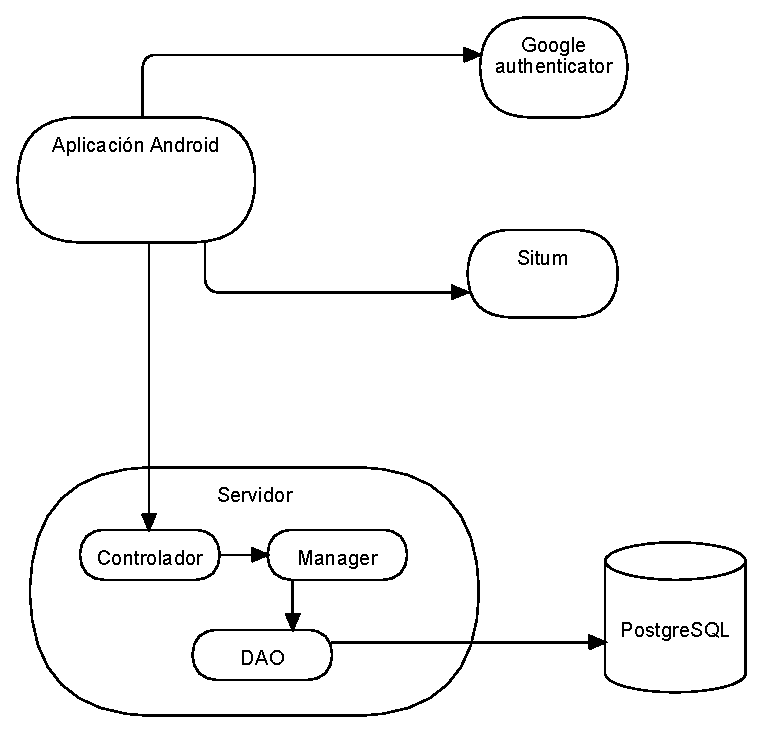
\includegraphics[width=0.65\textwidth]{figures/diagrama/arquitecturaGlobalSistema}
		\caption{Arquitectura xeral da plataforma Caronte para a guía de museos.}
		\label{fig:arq_xeral}
	\end{center}
\end{figure}

\paragraph{Servidor}
O servidor encárgase de recuperar e procesar a información que precisa a aplicación para o seu funcionamento. Esta información é almacenada nunha base de datos PostgreSQL. Aparte de recuperar esta información, tamén se encarga de inserir os datos indicados polo usuario dentro da aplicación. Para permitir a comunicación coa aplicación Android e que o usuario poida recibir e modificar esa información, publícanse uns servizos web a través dunha API REST. Decidiuse despregalo en Amazon Web Services por varios motivos, entre os cales se encontran:

\begin{itemize}
	\item Facilidade de configuración e uso, tanto para obter o propio servidor como para engadir novos elementos como pode ser a base de datos PostgreSQL.
	\item Escalabilidade.
	\item Rentabilidade.
	\item Seguridade.
\end{itemize}

\paragraph{Aplicación Android}
É o punto de interacción do usuario coa nosa plataforma. Presenta a información recuperada do servidor ao usuario e permite a súa modificación, enviando de novo os datos para a súa persistencia. Tamén é a encargada de tratar cos servizos de Situm que permiten a localización e o guiado en interiores, recuperando a información necesaria e presentándolla ao usuario.

\paragraph{Autenticación con Google}
O sistema de autenticación de Google permite a recuperación de información propia do usuario a través dunha conta de Google. Ao utilizar este sistema, pódese dispoñer da información dunha conta de usuario e gardala no noso servidor, polo que se pode utilizar para asociar permisos ou gardar outra información relacionada.


\section{Modelo de datos}
Neste punto exporase o modelo de datos da plataforma que se seguiu á hora da creación da base de datos. Na figura~\ref{fig:modelo_datos} pódese observar o diagrama entidade relación. Dividirase a explicación en base ás entidades.

\begin{figure}[tbh] 
	\begin{center}
		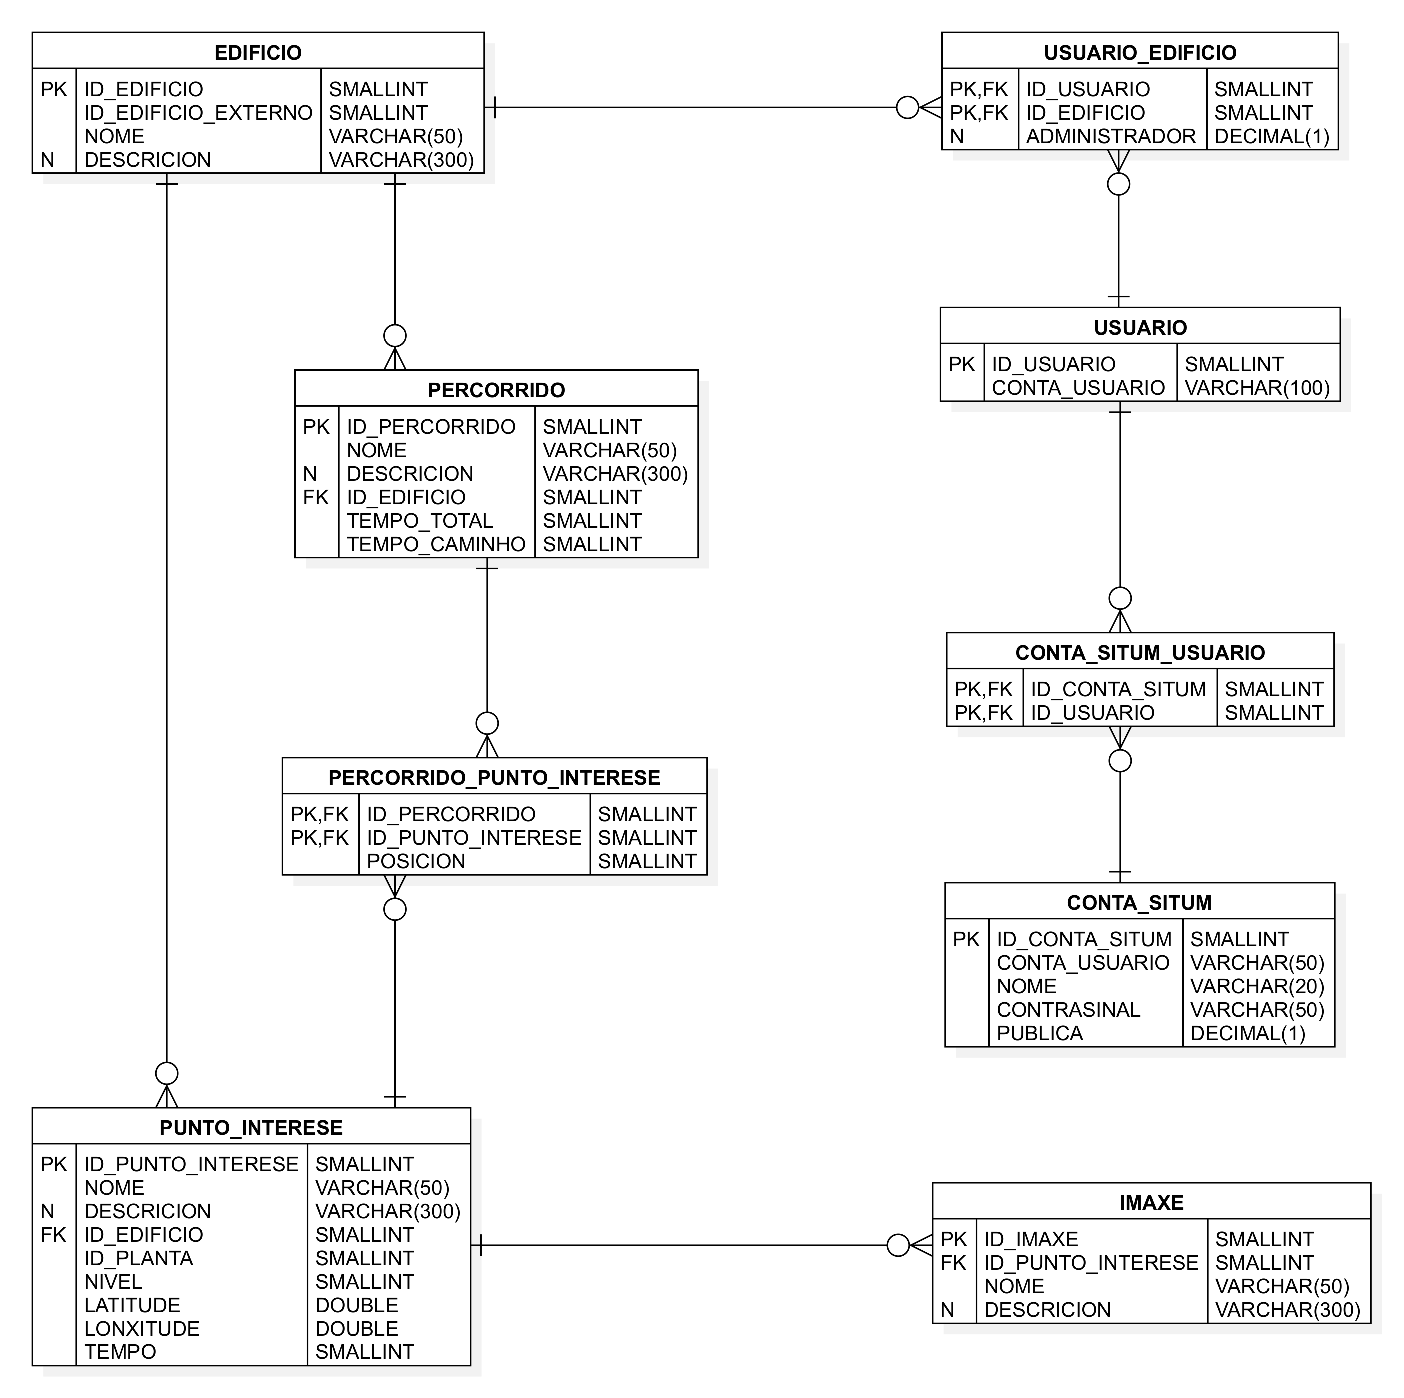
\includegraphics[width=0.75\textwidth]{figures/BD/diagramaEntidadeRelacion}
		\caption{Modelo de datos da plataforma Caronte.}
		\label{fig:modelo_datos}
	\end{center}
\end{figure}

\subsection{EDIFICIO}
Nesta entidade gardarase a información básica dos edificios que se tratan na aplicación. Aparte dos datos propios creados para a plataforma tamén se garda o identificador do edificio dentro do sistema Situm, que permite relacionar os edificios de Caronte cos de Situm.

As columnas das que se compón este entidade son:
\begin{itemize}
	\item ID\_EDIFICIO: Chave primaria autoxerada da táboa. De tipo SMALLINT (short). É o identificador do edificio dentro do sistema de Caronte. Non pode ter valor nulo.
	\item ID\_EDIFICIO\_EXTERNO: De tipo SMALLINT (short). É o identificador do edificio dentro do sistema de Situm.
	\item NOME: De tipo VARCHAR (string) con límite de 50 caracteres. É o texto que se visualizará na aplicación e que permite ao usuario a distinción entre edificios. Non pode ter valor nulo.
	\item DESCRICION: De tipo VARCHAR (string) con límite de 300 caracteres. Un breve texto explicativo sobre o edificio. Pode ter valor nulo.
\end{itemize}

\subsection{USUARIO}
Nesta entidade gardarase a conta de usuario de Google coa que alguén se autentica na aplicación. Só se gardará o nome desa conta.

As columnas das que se compón este entidade son:
\begin{itemize}
	\item ID\_USUARIO: Chave primaria autoxerada da táboa. De tipo SMALLINT (short). É o identificador do usuario dentro do sistema de Caronte. Non pode ter valor nulo.
	\item CONTA\_USUARIO: De tipo VARCHAR (string) con límite de 100 caracteres. Correspóndese coa conta de correo de Google do usuario que se autentica na aplicación. Non pode ter valor nulo.
\end{itemize}

\subsection{USUARIO\_EDIFICIO}
Nesta entidade gardarase información sobre as accións que pode levar a cabo un usuario sobre un edificio concreto. A información desta entidade é a que indica se un usuario é un xestor de contido sobre un edificio e será inserida polo Administrador do sistema.

As columnas das que se compón este entidade son:
\begin{itemize}
	\item ID\_USUARIO: Forma parte da chave primaria da entidade. Chave foránea da táboa USUARIO. De tipo SMALLINT (short). Non pode ter valor nulo.
	\item ID\_EDIFICIO: Forma parte da chave primaria da entidade. Chave foránea da táboa EDIFICIO. De tipo SMALLINT (short). Non pode ter valor nulo.
	\item ADMINISTRADOR: De tipo DECIMAL con límite 1 (boolean). Indica se o usuario é xestor de contido sobre o edificio.
\end{itemize}


\subsection{PUNTO\_INTERESE}
Nesta entidade gardarase información sobre os puntos de interese creados sobre un edificio e a súa localización exacta no planeta en base a coordenadas. Un punto de interese só pode pertencer a un único edificio e estará localizado nunha das súas plantas. Serán creados a través da aplicación polos Xestores de contido.

As columnas das que se compón este entidade son:
\begin{itemize}
	\item ID\_PUNTO\_INTERESE: Chave primaria autoxerada da táboa. De tipo SMALLINT (short). É o identificador do punto de interese. Non pode ter valor nulo.
	\item NOME: De tipo VARCHAR (string) con límite de 50 caracteres. É o texto que se visualizará na aplicación e que permite ao usuario a distinción entre puntos de interese. Non pode ter valor nulo.
	\item DESCRICION: De tipo VARCHAR (string) con límite de 300 caracteres. Un breve texto explicativo sobre o punto de interese. Pode ter valor nulo.
	\item ID\_EDIFICIO: Chave foránea da táboa EDIFICIO. De tipo SMALLINT (short). Permite identificar o edificio no que se atopa o punto. Non pode ter valor nulo.
	\item ID\_PLANTA: De tipo SMALLINT (short). É o identificador da planta dentro do sistema de Situm. Este dato permite maior rapidez á hora de identificador os puntos dunha planta. Non pode ter valor nulo.
	\item NIVEL: De tipo SMALLINT (short). Indica o número de planta no que se atopa un punto. Non pode ter valor nulo.
	\item LATITUDE: De tipo DOUBLE. Indica a latitude do punto, o que permite unha localización exacta nun mapa. Non pode ter valor nulo.
	\item LONXITUDE: De tipo DOUBLE. Indica a lonxitude do punto, o que permite unha localización exacta nun mapa. Non pode ter valor nulo.
	\item TEMPO: De tipo SMALLINT (short). Indica o tempo en minutos de media que lle leva a un visitante admirar unha obra. Non pode ter valor nulo e o seu valor por defecto é 0.
\end{itemize}


\subsection{PERCORRIDO}
Nesta entidade gardarase información sobre os percorridos dispoñíbeis nos edificios. Un percorrido só pode pertencer a un único edificio e non está limitado a unha única planta. Está composto por varios puntos de interese que se almacenan na táboa do seguinte punto. Serán creados a través da aplicación polos Xestores de contido.

As columnas das que se compón este entidade son:
\begin{itemize}
	\item ID\_PERCORRIDO: Chave primaria autoxerada da táboa. De tipo SMALLINT (short). É o identificador do percorrido. Non pode ter valor nulo.
	\item NOME: De tipo VARCHAR (string) con límite de 50 caracteres. É o texto que se visualizará na aplicación e que permite ao usuario a distinción entre percorridos. Non pode ter valor nulo.
	\item DESCRICION: De tipo VARCHAR (string) con límite de 300 caracteres. Un breve texto explicativo sobre o percorrido. Pode ter valor nulo.
	\item ID\_EDIFICIO: Chave foránea da táboa EDIFICIO. De tipo SMALLINT (short). Permite identificar o edificio no que se atopa o percorrido. Non pode ter valor nulo.
	\item TEMPO\_TOTAL: De tipo SMALLINT (short). Indica o tempo en minutos de media que lle leva a un visitante realizar todo o percorrido contando co tempo que pase diante das obras. Non pode ter valor nulo e o seu valor por defecto é 0.
	\item TEMPO\_CAMINHO: De tipo SMALLINT (short). Indica o tempo en minutos de media que lle leva a un visitante realizar todo o percorrido sen contar o tempo que pase diante das obras. Non pode ter valor nulo e o seu valor por defecto é 0.
\end{itemize}


\subsection{PERCORRIDO\_PUNTO\_INTERESE}
Nesta entidade gardarase a relación entre os percorridos e os puntos de interese que os compoñen. É obrigatorio indicar a posición de cada un deses puntos dentro do percorrido xa que ten unha orde establecida. Un punto de interese só pode aparecer unha única vez nun percorrido, non se permite a súa repetición. Non hai limitación no numero de percorridos aos que pode pertencer un punto de interese.

As columnas das que se compón este entidade son:
\begin{itemize}
	\item ID\_PERCORRIDO: Forma parte da chave primaria da entidade. Chave foránea da táboa PERCORRIDO. De tipo SMALLINT (short). Non pode ter valor nulo.
	\item ID\_PUNTO\_INTERESE: Forma parte da chave primaria da entidade. Chave foránea da táboa PUNTO\_INTERESE. De tipo SMALLINT (short). Non pode ter valor nulo.
	\item POSICION: De tipo SMALLINT (short). Indica a posición ordenada dun punto de interese dentro dun percorrido. Non pode ter valor nulo.
\end{itemize}


\subsection{CONTA\_SITUM}
Nesta entidade almacénanse as distintas contas de usuario dispoñíbeis na aplicación para o acceso á plataforma de Situm. Con elas permítese a visión de distintos edificios e o seu tratamento na aplicación. As contas poden ser públicas ou privadas, precisando certo permiso o usuario para poder visualizar estas últimas. A indicación de se unha conta é publica ou privada decídeo o Administrador do sistema.

As columnas das que se compón este entidade son:
\begin{itemize}
	\item ID\_CONTA\_SITUM: Chave primaria autoxerada da táboa. De tipo SMALLINT (short). É o identificador da conta de Situm. Non pode ter valor nulo.
	\item CONTA\_USUARIO: De tipo VARCHAR (string) con límite de 50 caracteres. É o correo electrónico que utiliza Situm para autenticarse. Non pode ter valor nulo.
	\item NOME: De tipo VARCHAR (string) con límite de 20 caracteres. É o texto que se visualizará na aplicación e que permite ao usuario a distinción entre contas de Situm. Non pode ter valor nulo.
	\item CONTRASINAL: De tipo VARCHAR (string) con límite de 50 caracteres. É o contrasinal que permite a conexión ao sistema de Situm. Non pode ter valor nulo.
	\item PUBLICA: De tipo DECIMAL con límite 1 (boolean). Indica se a conta de Situm pode ser por calquera usuario ou en cambio debe ter permisos sobre ela. Non pode ter valor nulo.
\end{itemize}


\subsection{CONTA\_SITUM\_USUARIO}
Nesta entidade almacénanse as relacións entre os usuarios e as distintas contas de acceso a Situm sobre as que teñen permiso. Non almacena máis que esa relación. Se o usuario ten algunha conta asociada poderá utilizala para acceder ao sistema. Estas relacións establéceas o Administrador do sistema.

As columnas das que se compón este entidade son:
\begin{itemize}
	\item ID\_CONTA\_SITUM: Forma parte da chave primaria da entidade. Chave foránea da táboa CONTA\_SITUM. De tipo SMALLINT (short). Non pode ter valor nulo.
	\item ID\_USUARIO: Forma parte da chave primaria da entidade. Chave foránea da táboa USUARIO. De tipo SMALLINT (short). Non pode ter valor nulo.
\end{itemize}


\subsection{IMAXE}
Nesta entidade almacénase a información sobre todas as imaxes subidas. Cada rexistro debe facer referencia a un punto de interese concreto. A propia imaxe non é almacenada nesta táboa, senón que se gardará no servidor. A información almacenada nesta táboa permitirá a identificación da ruta creada para recuperar a imaxe. As imaxes son engadidas polos Xestores de contido.

As columnas das que se compón este entidade son:
\begin{itemize}
	\item ID\_IMAXE: Chave primaria autoxerada da táboa. De tipo SMALLINT (short). É o identificador da imaxe. Non pode ter valor nulo.
	\item ID\_PUNTO\_INTERESE: Chave foránea da táboa PUNTO\_INTERESE. De tipo SMALLINT (short). Permite identificar o punto de interese ao que fai referencia a imaxe. Non pode ter valor nulo.
	\item NOME: De tipo VARCHAR (string) con límite de 50 caracteres. É o texto que se visualizará na aplicación e que permite ao usuario a distinción entre imaxes. Non pode ter valor nulo.
	\item DESCRICION: De tipo VARCHAR (string) con límite de 300 caracteres. Un breve texto explicativo sobre a imaxe. Pode ter valor nulo.
\end{itemize}


\section{Servidor}
Nesta sección describiremos as decisións máis importantes tomadas no deseño do servidor. No primeiro punto explícanse as capas nas que se dividiu o servidor e o obxectivo de cada unha delas. Nos seguintes puntos expóñense as opcións levadas a cabo para a definición do servizo web ou a transaccionalidade, entre outras.

\begin{figure}[tbh] 
	\begin{center}
		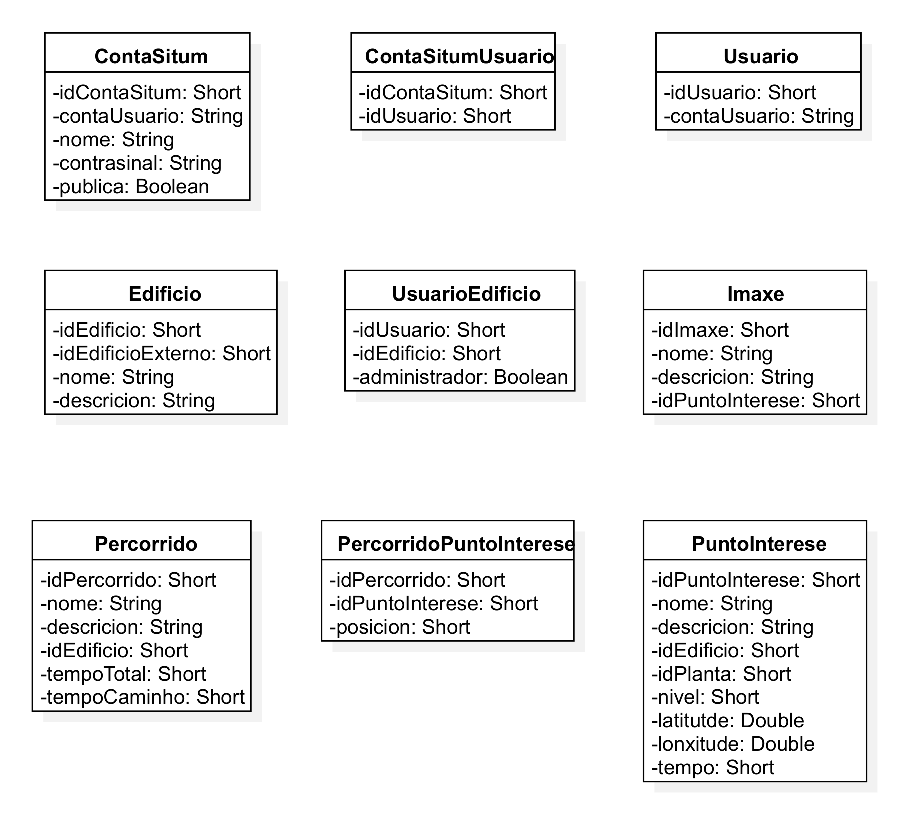
\includegraphics[width=0.70\textwidth]{figures/Clases/diagramaEntidades}
		\caption{Diagrama de clases coas entidades.}
		\label{fig:entidades}
	\end{center}
\end{figure}

\subsection{División en capas}
O servidor divídese nunha serie de capas que se diferencian no obxectivo que perseguen. Na figura~\ref{fig:arq_xeral} pódense ver dentro do servidor e como interactúan entre elas. As capas do servidor son as seguintes:

\begin{itemize}
	\item Entidade: A representación da información recuperada da base de datos faise mediante certas clases denominadas entidades. Non teñen lóxica, só se utilizan para o almacenamento de datos. Poden utilizarse en todas as capas do servidor. Pódense observar na figura ~\ref{fig:entidades}.
	\item DAO: Capa de acceso a datos. Nesta capa prodúcese a recuperación da información de base de datos, así como a súa inserción, borrado e modificación a través das entidades. Esta capa está ausente de toda lóxica de tratamento destes datos, limítase á realización das accións comentadas, deixando os trámites ás capas superiores. Pódense observar na figura ~\ref{fig:daos}.
	\item Manager: Encárgase da xestión dos datos. Se no tratamento da información se precisa unha combinación entre os datos recuperados de distintos puntos é aquí onde se realiza. Nesta capa é onde se implementa a transaccionalidade, polo que se ocorre un erro durante a execución dun método dentro do manager que realiza cambios en base de datos, desfai as modificacións previas realizadas en BD para que a información quede consistente.
	\item Controlador: Encárgase da comunicación a través dos servizos web. Implementa a API REST que permite o acceso aos servizos.
\end{itemize}



\begin{figure}[tbh] 
	\begin{center}
		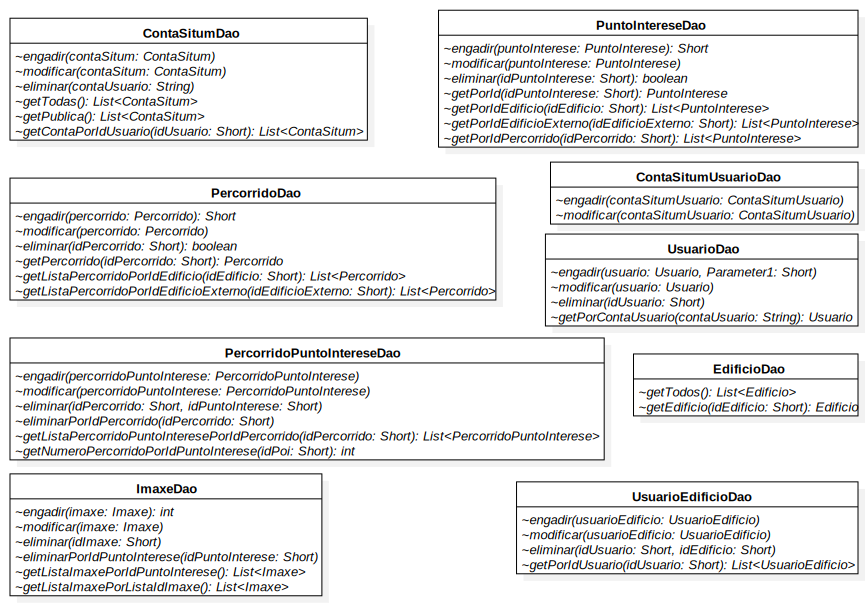
\includegraphics[width=0.90\textwidth]{figures/BD/daos}
		\caption{Diagrama de clases cos DAOs.}
		\label{fig:daos}
	\end{center}
\end{figure}


\subsection{Transaccionalidade}
Ningunha aplicación está libre de que se produza algún erro na súa execución, ben sexa por culpa de erros na implementación ou por elementos externos (caídas de conexións, erros na base de datos, etc...), polo que é preciso ter en conta estas situacións á hora de realizar modificacións sobre a base de datos para evitar a existencia de información errónea. Cando se realizan modificacións en serie sobre a base de datos que requiren da intervención de varias táboas pode ocorrer un erro xusto no medio, provocando que algunhas táboas fosen modificadas e outras non. Neste caso romperíase a integridade dos datos. Para evitar isto, búscase un sistema que permita que se realicen esas modificacións como se fosen unha soa, e no caso de que se produza un erro, que se desfagan os cambios.

\begin{table} [tbh]
	\footnotesize
	\centering
	\begin{tabular}{|l|p{5cm}|p{7cm}|}
		\hline 
		\textbf{Método}	& \textbf{Dirección} & \textbf{Descrición} \\ 
		\hline 
		GET & /recuperar/(idEd)/(idPoi)/(idIm) & Recupera a imaxe indicada polo id=(idIm) do poi con id=(idPoi) do edificio=(idEd) \\ 
		\hline 
		POST & /subir & Envía unha imaxe para un POI dun edificio concreto, engadindo nome e descrición \\ 
		\hline 
		POST & /actualizar/(idIm)/(nome)/(desc) & Actualiza a información, nome e descrición, da imaxe indicada polo id=(idIm) \\ 
		\hline 
		DELETE & /eliminar/(idIm) & Elimina a imaxe indicada polo id=(idIm) \\ 
		\hline 
	\end{tabular}
	\caption{Descricións da API Rest para o tratamento de imaxes.}
	\label{tab:APIImaxes}
\end{table}

\subsection{API REST}
A API utilizada para os servizos web é REST, polo que o formato dos datos enviados e recibidos son, na súa maioría JSON. A única excepción prodúcese no envío de imaxes. As respostas producidas polos servizos tamén serán devoltas no mesmo formato.
A API foi dividida en dúas seccións, por unha parte a relacionada coas imaxes (envío, recepción e modificación de datos) e por outra a relacionada co resto de elementos do sistemas (POIs, edificios, percorridos). O tratamento de imaxes é un servizo que é susceptíbel de ser modificado para levalo a cabo por outro métodos xa que pode ter un alto consumo de datos. Desta maneira limítase o impacto que tería unha modificación neste aspecto dentro dos nosos servizos se se queren utilizar cachés propias para imaxes.

Todas as URLs comezan por \emph{/sw} mais a continuación dependen da sección á cal pertenzan: se son da información xeral levarán a continuación \emph{/museo}, mentres que as de tratamento de imaxes levarán \emph{/imaxe}. Un exemplo de URL de cada sección:

\begin{itemize}
	\item http://\emph{direccionSW}:\emph{porto}/sw/museo/contas/\emph{(idUsuario)}
	\item http://\emph{direccionSW}:\emph{porto}/sw/imaxe/recuperar/\emph{(idEdificio)}/\emph{(idPoi)}/\emph{(idImaxe)}
\end{itemize}

Os parénteses fan referencia a variábeis dentro das chamadas, texto que non é fixo senón que varía dependendo dos datos que queira solicitar o usuario.

Nas táboas poden observarse todas as chamadas dispoñíbeis dentro dos servizos web e as súas características, tanto para as imaxes (táboa \ref{tab:APIImaxes}) coma para o resto de información (táboa \ref{tab:APIXeral}).

\begin{table} [!h]
	\footnotesize
	\centering
	\begin{tabular}{|l|p{5cm}|p{7cm}|}
		\hline 
		\textbf{Método}	& \textbf{Dirección} & \textbf{Descrición} \\ 
		\hline 
		GET & /edificios & Recupera todos os edificios \\ 
		\hline 
		GET & /pois/(idEdificioExterno) & Recupera todos os POIs do edificio con id externo=(idEdificioExterno) \\ 
		\hline 
		GET & /contas & Recupera todas as contas de Situm públicas \\ 
		\hline 
		GET & /contas/(idUsuario) & Recupera todas as contas de Situm ás que ten acceso o usuario con id=(idUsuario) \\ 
		\hline 
		GET & /percorridos/(idEd) & Recupera todos os percorridos do edificio con id=(idEdificio) \\ 
		\hline 
		GET & /percorridosidexterno/(idEdEx) & Recupera todos os percorridos do edificio con id externo=(idEdEx) \\ 
		\hline 
		GET & /ppi/(idPercorrido) & Recupera os puntos de interese do percorrido con id=(idPercorrido) \\ 
		\hline 
		POST & /percorrido/gardar & Garda os datos dun percorrido en BD \\ 
		\hline 
		POST & /comprobarUsuarioGoogle & Comproba que a autenticación a través da conta de Google do usuario é correcta \\ 
		\hline 
		POST & /poi/gardar & Garda os datos dun POI en BD \\ 
		\hline 
		DELETE & /percorrido/eliminar/(idPercorrido) & Elimina un percorrido con id=(idPercorrido). Devolve un valor indicando o éxito \\ 
		\hline 
		DELETE & /poi/eliminar/(idPoi) & Elimina un POI con id=(idPoi). Devolve un valor indicando o éxito \\ 
		\hline 
		GET & /imaxe/recuperar/(IdImaxeCSV) & Recupera a información dunha lista de imaxes en CSV \\ 
		\hline 
	\end{tabular}
	\caption{Descricións da API Rest para o tratamento da información xeral.}
	\label{tab:APIXeral}
\end{table}

\subsection{Intercambio de datos}
O intercambio de datos entre a aplicación Android e o servidor faise en formato JSON. Na figura~\ref{fig:jsonRequest} pódese ver un exemplo de solicitude de creación dun punto de interese. A devolución dos datos tamén se realiza no mesmo formato. Un exemplo disto pódese observar na figura~\ref{fig:json}, onde se expón a resposta a unha chamada para a recuperación da información dos puntos de interese dun edificio.

\begin{figure}[tbh]
	\begin{center}
		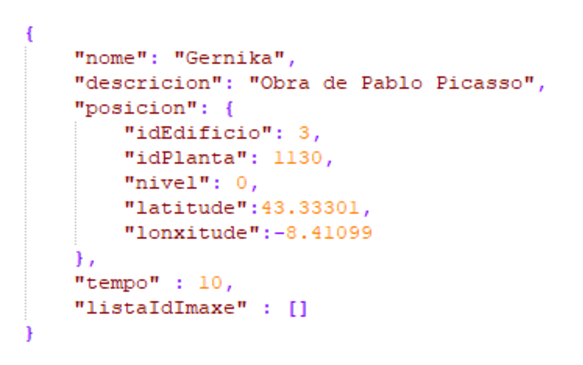
\includegraphics[width=0.55\textwidth]{figures/codigo/jsonRequest}
		\caption{Exemplo dunha solicitude ao servizo web.}
		\label{fig:jsonRequest}
	\end{center}
\end{figure}

\begin{figure}[tbh]
	\begin{center}
		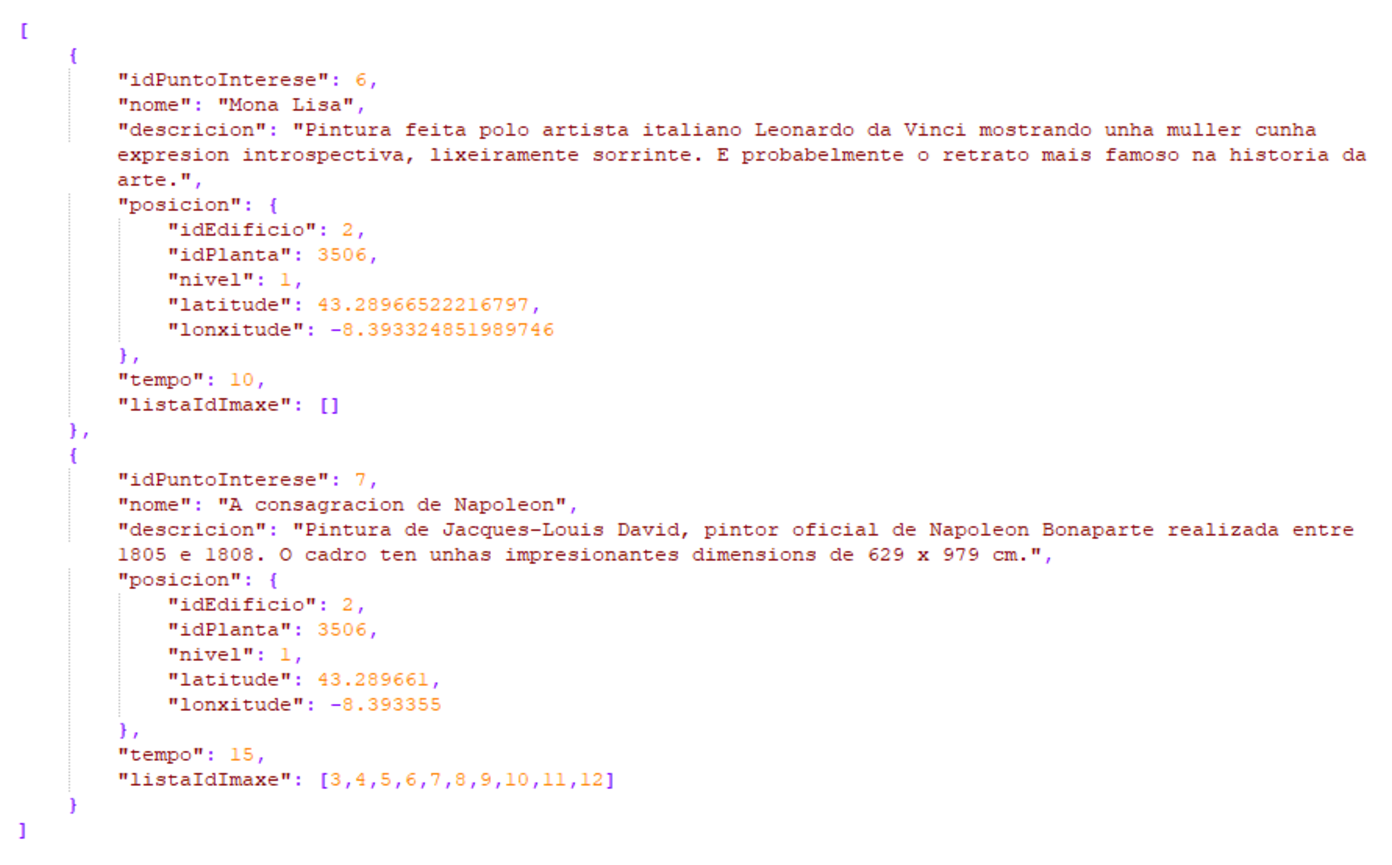
\includegraphics[width=1\textwidth]{figures/codigo/json}
		\caption{Exemplo dunha resposta do servizo web.}
		\label{fig:json}
	\end{center}
\end{figure}

En ambas figuras obsérvase a estrutura que caracteriza este formato de intercambio de datos. Outra das cuestións que nos permite observar é que a súa estrutura non coincide coa utilizada en base de datos, xa que as necesidades da aplicación non teñen por que coincidir coas decisións tomadas á hora de definir as táboas de base de datos. É por iso que se observa a agrupación da información sobre a localización física dos POIs nunha etiqueta chamada posición, que non coincide coa maneira de gardar eses valores en BD. A maiores tamén se inclúen os identificadores das imaxes almacenadas sobre cada POI, para simplificar a recuperación das imaxes na aplicación.

Para realizar a chamada ao servidor utilízase a librería spring-android-rest-template, que é o cliente para aplicacións Android de Spring \cite{springAndroid} que permite a realización de chamadas REST. Na sección de implementación describiranse exemplos da utilización desta librería.

Na parte do servidor tamén se utiliza Spring \cite{spring} mediante a librería spring-mvc, que se encarga de converter automaticamente as clases a formato JSON. Para isto débese incluir a dependencia de jackson-databind e indicar nas chamadas as etiquetas \lstinline{@RequestBody} e \lstinline{@ResponseBody}. Igual que para as chamadas dende Android, na sección de implementación amosarase algún exemplo desta configuración.

\subsection{Securización das comunicacións}
Tal e como se indicou no capítulo de conceptos teóricos, os servizos REST non teñen estado, polo que non se garda información ningunha entre peticións. É por isto que en cada petición se debe enviar toda a información para que se poida procesar, o que inclúe a información de securización.
Para a autenticación dos servizos utilizouse o sistema Basic, que consiste no envío dun usuario e contrasinal codificados en Base64. Na cabeceira da chamada REST aparecerá algo semellante ao texto da figura~\ref{fig:authorization}.

\begin{figure}[!h]
	\begin{center}
		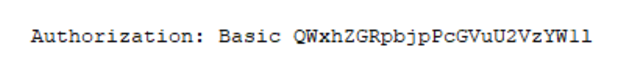
\includegraphics[width=0.6\textwidth]{figures/codigo/authorization}
		\caption{Exemplo dunha cabeceira REST securizada.}
		\label{fig:authorization}
	\end{center}
\end{figure}


\section{Sistema de autenticación a través de Google}
Debido á necesidade de distinguir os usuarios da aplicación entre os normais e os xestores de contido houbo que integrar un sistema de autenticación na aplicación, mais non se creou un propio.
Por motivos de comodidade e seguridade escolleuse a opción de realizar a autenticación dos usuarios a través de contas de Google, desta maneira non é preciso gardar información privada dos usuarios quedando estes datos do lado de Google. Ao estar destinada a aplicación ao sistema operativo Android non se obriga ao usuario a ter que crear unha conta ex profeso xa que é obrigatorio o uso dunha para poder utilizar un dispositivo móbil con Android.

\begin{figure}[!h]
	\begin{center}
		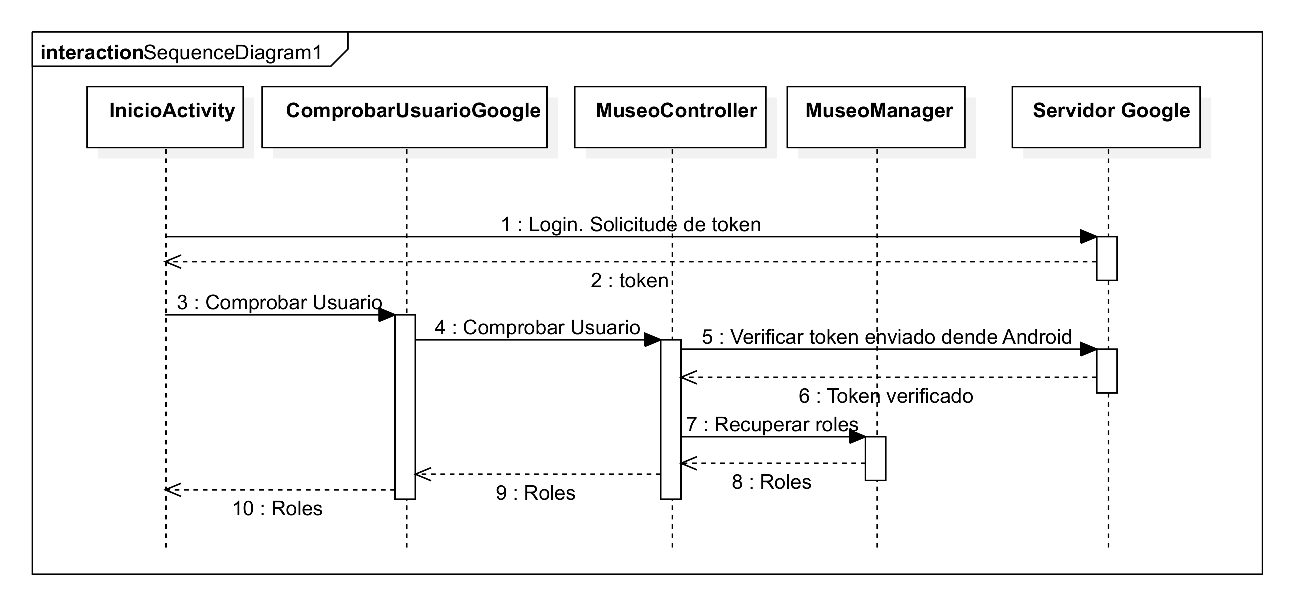
\includegraphics[width=1\textwidth]{figures/diagrama/secuenciaAutenticacionGoogle}
		\caption{Diagrama de secuencia da autenticación a través de Google.}
		\label{fig:secuenciaAutenticacionGoogle}
	\end{center}
\end{figure}

Para a integración do sistema de autenticación na aplicación hai que facer uso dos servizos de Google Play tanto no servidor coma na aplicación Android. É preciso configurar a aplicación para que permita a autenticación, acción que se fai a través dun formulario onde se indica o proxecto, o nome da aplicación e o seu tipo (Android, neste caso).

No diagrama da figura~\ref{fig:secuenciaAutenticacionGoogle} pode observarse o proceso de autenticación que se explica a continuación. Unha autenticación exitosa require de varios pasos. O primeiro é a autenticación dende a aplicación Android, dende a cal se enviarán os datos da conta a Google para que os verifique. Se os datos son correctos devólvese información sobre a conta á aplicación, para posteriormente enviar un token de sesión ao servidor que permita identificar ao usuario. No seguinte paso, o servidor recolle ese token e o envía de novo aos servizos de Google para verificar a súa integridade. Unha vez verificada, enviará a información sobre os roles dos que ese usuario dispón á aplicación Android para que poida utilizala coa conta seleccionada.

Os roles resultantes da autenticación a través da conta de Google poden permitir a modificación da información en certos edificios se ese usuario exerce como xestor de contido; noutro caso, actuará coma un usuario anónimo máis. Este rol de xestor de contido amosará un novo botón no mapa que permitirá ter acceso ao modo de edición, no que se mostrarán os botóns de creación e modificación de POIs e percorridos. Tamén dependen do usuario as contas de Situm dispoñíbeis, xa que é posíbel que algunha desas contas sexan privadas en vez de públicas e se outorguen permisos individualmente.

\section{Aplicación Android}
Escolleuse unha única aplicación tanto para a consulta como para a edición para aproveitar a potencia que nos dá o mapa de interiores á hora de localizar os puntos desexados e marcalos directamente. Desta maneira pódense situar con precisión os puntos sobre o mapa mentres se percorre o edificio. Non obstante, para unha futura ampliación do sistema sería interesante permitir a configuración dende un cliente web para a creación de contido referente aos puntos e os percorridos, xa que dende un dispositivo móbil non se obtén a mesma comodidade á hora de inserir textos e proporcionar información.

Procurouse realizar un deseño moi visual mediante a utilización de moitos botóns con imaxes na actividade do mapa para un mellor aproveitamento do espazo e un estilo máis clásico no resto de actividades que resultase menos rechamante pero máis cómodo. As cores principais da aplicación son o azul escuro sobre fondos brancos e maxenta coma cor secundaria.

\begin{figure}[H]
	\begin{center}
		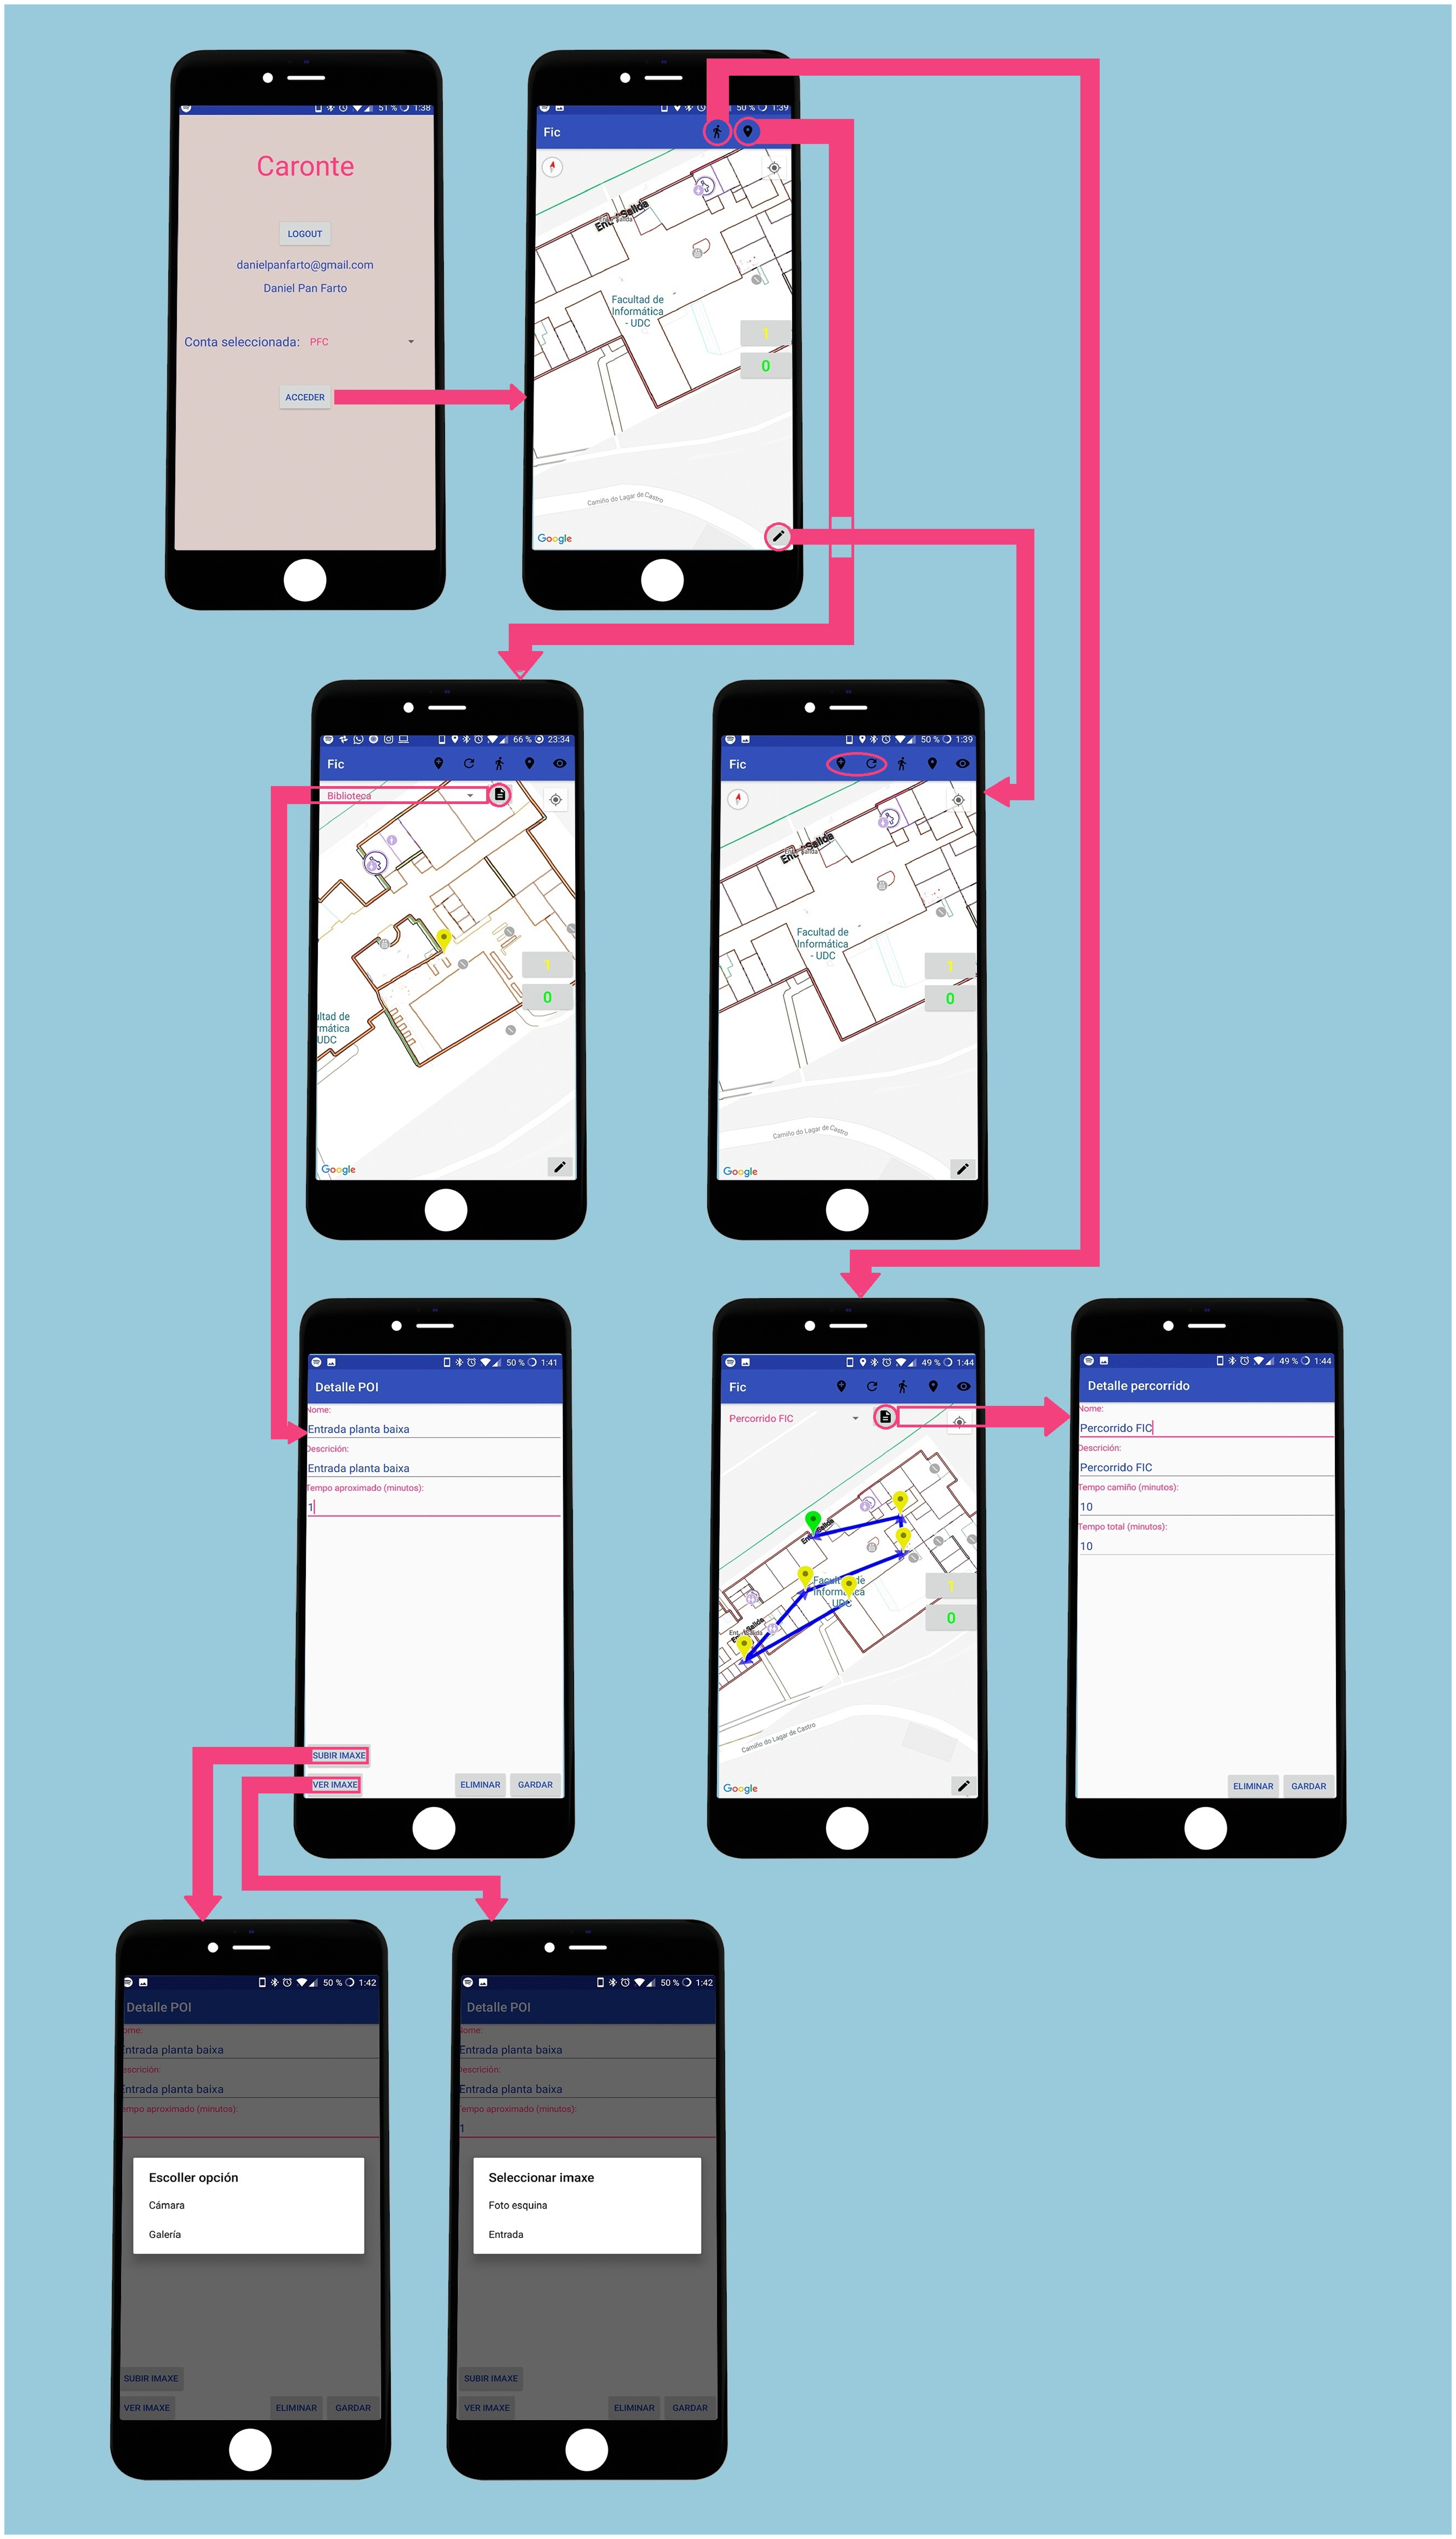
\includegraphics[width=0.85\textwidth]{figures/Capturas/fluxoAplicacion}
		\caption{Diagrama de fluxo da aplicación dende a pantalla de login ao resto de vistas.}
		\label{fig:fluxoAplicacion}
	\end{center}
\end{figure}

A estrutura de paquetes da aplicación é moi simple, separando as clases en cinco paquetes principais con base \emph{gal.caronte}:

\begin{itemize}
	\item activity: Neste paquete inclúense todas as actividades utilizadas na aplicación e que se explican no seguinte punto.
	\item custom: Obxectos propios da aplicación que se utilizan para transmitir datos entre actividades ou almacenar información recuperada do servidor. Estas últimas clases están almacenadas no paquete interno \emph{sw}.
	\item servizo: As clases nas que se producen as conexións contra o servidor ou contra Situm atópanse neste paquete.
	\item util: Clases de utilidades para tratar cadeas de texto, solicitar permisos ou outro tipo de accións que poden ser comúns en diversas clases.
	\item view: Elementos da vista que poderían utilizarse en varias actividades, coma o selector de POIs e percorridos.
\end{itemize}

\subsection{Actividades}
Unha das primeiras decisións á hora de crear unha aplicación Android débese tomar sobre a utilización ou non de fragmentos. Apostouse por unha aplicación que utilizase varias actividades cunha única excepción, o fragmento onde se mostra o mapa de Google Maps. Esta decisión adoptouse debido á maior complexidade que adquire o código co tratamento de fragmentos e o pouco proveito que se lles sacaría nesta aplicación.

A aplicación non ten un gran número de actividades debido a que case toda a lóxica recae sobre a actividade que contén o mapa e que supón o centro de toda actividade realizada na aplicación. A continuación describimos cada unha das actividades creadas.

A actividade inicial permite a autenticación a través de Google e a selección da conta de Situm utilizada que permitirá o acceso a certos edificios. As contas dispoñíbeis estarán restrinxidas en base á conta coa que se autentique o usuario, polo que non sempre se verán as mesmas. Hai algunhas que son públicas polo que estarán dispoñíbeis para todos os usuarios da aplicación. Se o usuario se autentica a través de Google pode dispoñer de permisos de xestor de contidos dentro dalgún edificio, polo que disporá de máis opcións no resto de actividades.


\begin{figure}[h]
	\begin{center}
		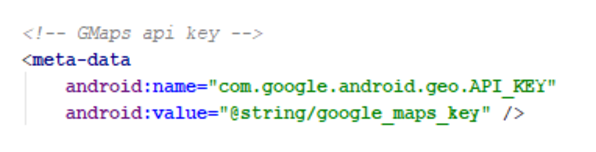
\includegraphics[width=0.6\textwidth]{figures/codigo/chaveGoogleMaps}
		\caption{Chave para o acceso a Google Maps.}
		\label{fig:chaveGoogleMaps}
	\end{center}
\end{figure}

A actividade na que se sitúa o mapa, como xa comentamos, é a principal, e ten por nome MapaActivity. O fragmento de Google Maps que amosa o noso mapa modificado atópase nesta actividade. Para poder utilizar Google Maps na aplicación houbo que activar unha chave na consola de Google Cloud \cite{chaveGoogleMaps} e incluíla no \emph{AndroidManifest}. Esta chave pódese observar na figura~\ref{fig:chaveGoogleMaps}. É a pantalla na que o usuario pasará máis tempo e onde se require amosar maior información, polo que tamén é a máis complexa. A maioría das accións levadas a cabo sobre a aplicación se realizarán sobre esta actividade, como a de visualizar puntos de interese e percorridos. Se o usuario dispón de permisos de xestor de contidos dentro dun edificio, habilitarase o botón de edición que lle permitirá crear, modificar e eliminar puntos de interese e percorridos a través de novos botóns na barra principal da aplicación.

Creáronse unha serie de actividades dirixidas a amosar certa información dos puntos de interese e percorridos dos edificios cunha estrutura semellante: DetallePoiActivity e DetallePercorridoActivity. Nelas obsérvanse os datos propios deses elementos, permitindo a súa modificación e borrado nos xa existentes, e tamén a súa creación no caso de non existir previamente se o usuario ten permisos para realizar esas accións (xestor de contido).

Dende a actividade DetallePoiActivity pódense visualizar imaxes dentro dos POIs se dispoñen delas, así coma subir novas imaxes se o usuario é xestor de contido. Pódense sacar novas fotos a través da cámara ou subir imaxes dende a galería do dispositivo.

Para engadir lóxica ao mapa optouse por externalizar certos compoñentes coma o selector de piso e os spinners de selección para os puntos de interese e os percorridos para desta maneira non sobrecargar a actividade.

Nalgunhas das actividades utilizáronse menús contextuais para ofrecer certas opcións ao usuario. A adición ou eliminación dos puntos de interese dentro dun percorrido, a escolla entre cámara e galería á hora de subir imaxes ou a selección da imaxe a visualizar son casos nos que se optou por esta opción posto que esas accións eran demasiado complexas para poder realizalas nun único paso.


\subsection{Comunicación co servidor}
Para acceder á información dispoñíbel no servidor utilízanse servizos web propios que devolven os datos en formato JSON. As clases que se utilizan para comunicar esta información non teñen equivalencia exacta cos VOs, polo que hai que facer conversións antes de enviala e despois de recibila. Estas clases tamén se utilizan na aplicación Android.

A comunicación co servidor realízase mediante a librería de Spring adaptada a Android: spring-android-rest-template. Cada chamada realízase dende unha clase distinta para identificar mellor que fai cada unha delas. No apartado de implementación amosarase a creación destas chamadas.

Tal e como se comentou no apartado de "Securización das comunicacións", as chamadas precisan do envío dun token que permita o acceso aos servizos. Na sección de implementación poderá observarse como se engaden estes datos á cabeceira da solicitude.


\subsection{Comunicación con Situm}
Todo acceso realizado sobre o sistema de Situm prodúcese dende a aplicación móbil. O noso servidor non pode ter acceso ao sistema de Situm, polo que toda a información proporcionada sobre a localización que se precise no servidor debe ser enviada pola aplicación Android. Esta comunicación que se produce co sistema de Situm é en base ás credenciais que escolla o usuario, xa sexan públicas ou privadas.

No paquete gal.caronte.servizo.situm atópanse as clases que realizan as chamadas aos servidores de Situm. Cada chamada permitida a Situm realízase dende unha clase distinta, igual que se fixo coas comunicacións co servidor propio, para desta maneira identificar mellor que se fai dentro de cada unha delas.

Utilízase a librería proporcionada por Situm para realizar as chamadas \cite{situmDevelopers}. O acceso a esta librería indícase no ficheiro \emph{build.gradle} onde se fai referencia á dependencia \emph{es.situm:situm-sdk:2.9.0@aar}. No apartado de implementación explicarase a realización das solicitudes a Situm.

\subsection{Permisos necesarios}
A inmensa maioría de aplicacións en Android precisan dunha lista concreta de permisos que son necesarios para unha correcta execución ou para obter unha experiencia completa. Actualmente non se require a aceptación dos permisos na instalación, senón que poden concederse individualmente durante a execución da mesma.

Débense distinguir entre os permisos para os que fan falla unha aprobación explícita dos que van implícitos na execución. O caso do permiso sobre internet é un do segundo tipo, xa que ao estar tan estendido o seu uso, nas novas versións de Android non é preciso a súa aprobación.

A continuación describiranse os motivos polos que se solicitan cada un dos permisos da aplicación. O permiso \emph{ACCESS\_FINE\_LOCATION} requírese para un posicionamento axustado na utilización do mapa, polo que se non se acepta non se podería utilizar correctamente a aplicación. Os outros tres permisos solicítanse se se quere facer uso das imaxes dentro da aplicación, xa sexa para sacar fotos de POIs (\emph{CAMERA}), para acceder ás imaxes da galería do dispositivo (\emph{READ\_INTERNAL\_STORAGE}) ou para visualizar algunha imaxe dun POI (\emph{WRITE\_EXTERNAL\_STORAGE}, para gardala temporalmente).
